\documentclass{extbook}[14pt]
\usepackage{multicol, enumerate, enumitem, hyperref, color, soul, setspace, parskip, fancyhdr, amssymb, amsthm, amsmath, latexsym, units, mathtools}
\everymath{\displaystyle}
\usepackage[headsep=0.5cm,headheight=0cm, left=1 in,right= 1 in,top= 1 in,bottom= 1 in]{geometry}
\usepackage{dashrule}  % Package to use the command below to create lines between items
\newcommand{\litem}[1]{\item #1

\rule{\textwidth}{0.4pt}}
\pagestyle{fancy}
\lhead{}
\chead{Answer Key for Progress Quiz 8 Version A}
\rhead{}
\lfoot{5493-4176}
\cfoot{}
\rfoot{Summer C 2021}
\begin{document}
\textbf{This key should allow you to understand why you choose the option you did (beyond just getting a question right or wrong). \href{https://xronos.clas.ufl.edu/mac1105spring2020/courseDescriptionAndMisc/Exams/LearningFromResults}{More instructions on how to use this key can be found here}.}

\textbf{If you have a suggestion to make the keys better, \href{https://forms.gle/CZkbZmPbC9XALEE88}{please fill out the short survey here}.}

\textit{Note: This key is auto-generated and may contain issues and/or errors. The keys are reviewed after each exam to ensure grading is done accurately. If there are issues (like duplicate options), they are noted in the offline gradebook. The keys are a work-in-progress to give students as many resources to improve as possible.}

\rule{\textwidth}{0.4pt}

\begin{enumerate}\litem{
Construct the lowest-degree polynomial given the zeros below. Then, choose the intervals that contain the coefficients of the polynomial in the form $ax^3+bx^2+cx+d$.
\[ \frac{-4}{3}, \frac{4}{5}, \text{ and } \frac{6}{5} \]The solution is \( 75x^{3} -50 x^{2} -128 x + 96 \), which is option A.\begin{enumerate}[label=\Alph*.]
\item \( a \in [70, 77], b \in [-53, -41], c \in [-130, -119], \text{ and } d \in [86, 98] \)

* $75x^{3} -50 x^{2} -128 x + 96$, which is the correct option.
\item \( a \in [70, 77], b \in [50, 55], c \in [-130, -119], \text{ and } d \in [-100, -88] \)

$75x^{3} +50 x^{2} -128 x -96$, which corresponds to multiplying out $(3x -4)(5x + 4)(5x + 6)$.
\item \( a \in [70, 77], b \in [-53, -41], c \in [-130, -119], \text{ and } d \in [-100, -88] \)

$75x^{3} -50 x^{2} -128 x -96$, which corresponds to multiplying everything correctly except the constant term.
\item \( a \in [70, 77], b \in [-251, -249], c \in [271, 273], \text{ and } d \in [-100, -88] \)

$75x^{3} -250 x^{2} +272 x -96$, which corresponds to multiplying out $(3x -4)(5x -4)(5x -6)$.
\item \( a \in [70, 77], b \in [-131, -126], c \in [-33, -27], \text{ and } d \in [86, 98] \)

$75x^{3} -130 x^{2} -32 x + 96$, which corresponds to multiplying out $(3x -4)(5x + 4)(5x -6)$.
\end{enumerate}

\textbf{General Comment:} To construct the lowest-degree polynomial, you want to multiply out $(3x + 4)(5x -4)(5x -6)$
}
\litem{
Describe the end behavior of the polynomial below.
\[ f(x) = 5(x - 7)^{4}(x + 7)^{5}(x - 4)^{3}(x + 4)^{3} \]The solution is the graph below, which is option D.
    \begin{center}
        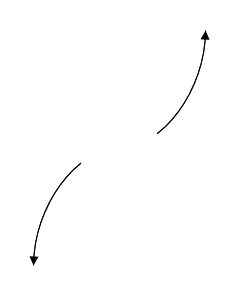
\includegraphics[width=0.3\textwidth]{../Figures/polyEndBehaviorCopyDA.png}
    \end{center}\begin{enumerate}[label=\Alph*.]
\begin{multicols}{2}
\item 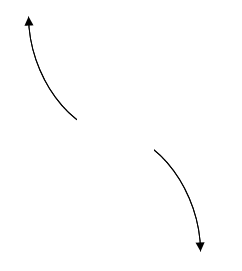
\includegraphics[width = 0.3\textwidth]{../Figures/polyEndBehaviorCopyAA.png}
\item 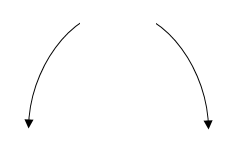
\includegraphics[width = 0.3\textwidth]{../Figures/polyEndBehaviorCopyBA.png}
\item 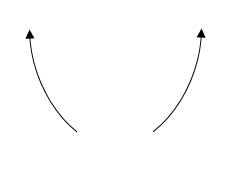
\includegraphics[width = 0.3\textwidth]{../Figures/polyEndBehaviorCopyCA.png}
\item 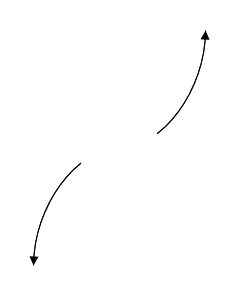
\includegraphics[width = 0.3\textwidth]{../Figures/polyEndBehaviorCopyDA.png}
\end{multicols}\item None of the above.\end{enumerate}
\textbf{General Comment:} Remember that end behavior is determined by the leading coefficient AND whether the \textbf{sum} of the multiplicities is positive or negative.
}
\litem{
Construct the lowest-degree polynomial given the zeros below. Then, choose the intervals that contain the coefficients of the polynomial in the form $x^3+bx^2+cx+d$.
\[ -2 + 4 i \text{ and } 1 \]The solution is \( x^{3} +3 x^{2} +16 x -20 \), which is option D.\begin{enumerate}[label=\Alph*.]
\item \( b \in [0.7, 1.4], c \in [-6, -3], \text{ and } d \in [2, 11] \)

$x^{3} + x^{2} -5 x + 4$, which corresponds to multiplying out $(x -4)(x -1)$.
\item \( b \in [0.7, 1.4], c \in [-1, 5], \text{ and } d \in [-9, 0] \)

$x^{3} + x^{2} +x -2$, which corresponds to multiplying out $(x + 2)(x -1)$.
\item \( b \in [-6.9, -1.6], c \in [14, 23], \text{ and } d \in [13, 26] \)

$x^{3} -3 x^{2} +16 x + 20$, which corresponds to multiplying out $(x-(-2 + 4 i))(x-(-2 - 4 i))(x + 1)$.
\item \( b \in [1.6, 6.2], c \in [14, 23], \text{ and } d \in [-25, -14] \)

* $x^{3} +3 x^{2} +16 x -20$, which is the correct option.
\item \( \text{None of the above.} \)

This corresponds to making an unanticipated error or not understanding how to use nonreal complex numbers to create the lowest-degree polynomial. If you chose this and are not sure what you did wrong, please contact the coordinator for help.
\end{enumerate}

\textbf{General Comment:} Remember that the conjugate of $a+bi$ is $a-bi$. Since these zeros always come in pairs, we need to multiply out $(x-(-2 + 4 i))(x-(-2 - 4 i))(x-(1))$.
}
\litem{
Describe the end behavior of the polynomial below.
\[ f(x) = -4(x - 4)^{5}(x + 4)^{10}(x + 6)^{3}(x - 6)^{5} \]The solution is the graph below, which is option A.
    \begin{center}
        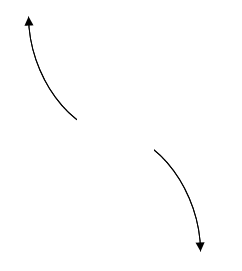
\includegraphics[width=0.3\textwidth]{../Figures/polyEndBehaviorAA.png}
    \end{center}\begin{enumerate}[label=\Alph*.]
\begin{multicols}{2}
\item 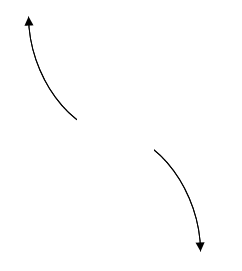
\includegraphics[width = 0.3\textwidth]{../Figures/polyEndBehaviorAA.png}
\item 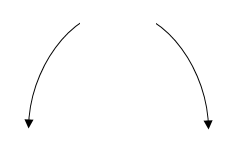
\includegraphics[width = 0.3\textwidth]{../Figures/polyEndBehaviorBA.png}
\item 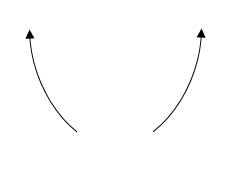
\includegraphics[width = 0.3\textwidth]{../Figures/polyEndBehaviorCA.png}
\item 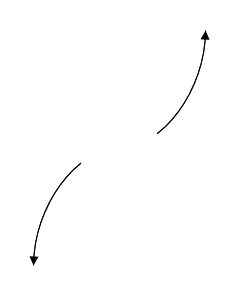
\includegraphics[width = 0.3\textwidth]{../Figures/polyEndBehaviorDA.png}
\end{multicols}\item None of the above.\end{enumerate}
\textbf{General Comment:} Remember that end behavior is determined by the leading coefficient AND whether the \textbf{sum} of the multiplicities is positive or negative.
}
\litem{
Which of the following equations \textit{could} be of the graph presented below?

\begin{center}
    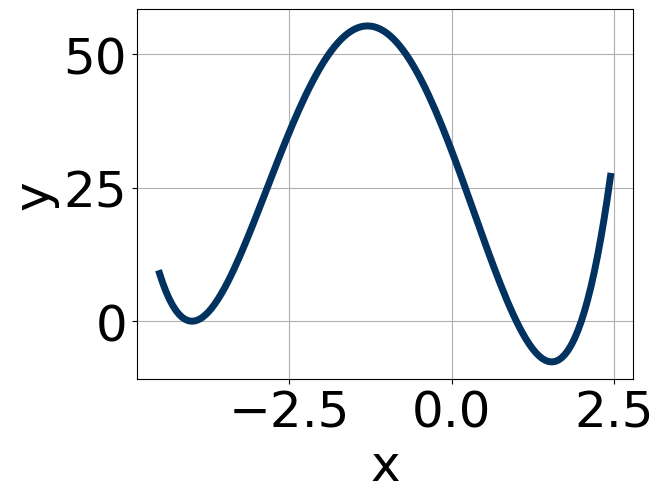
\includegraphics[width=0.5\textwidth]{../Figures/polyGraphToFunctionCopyA.png}
\end{center}


The solution is \( 10(x + 4)^{6} (x - 1)^{11} (x - 2)^{5} \), which is option A.\begin{enumerate}[label=\Alph*.]
\item \( 10(x + 4)^{6} (x - 1)^{11} (x - 2)^{5} \)

* This is the correct option.
\item \( 10(x + 4)^{8} (x - 1)^{10} (x - 2)^{5} \)

The factor $(x - 1)$ should have an odd power.
\item \( -12(x + 4)^{4} (x - 1)^{5} (x - 2)^{8} \)

The factor $(x - 2)$ should have an odd power and the leading coefficient should be the opposite sign.
\item \( -6(x + 4)^{10} (x - 1)^{11} (x - 2)^{11} \)

This corresponds to the leading coefficient being the opposite value than it should be.
\item \( 17(x + 4)^{7} (x - 1)^{10} (x - 2)^{5} \)

The factor $-4$ should have an even power and the factor $1$ should have an odd power.
\end{enumerate}

\textbf{General Comment:} General Comments: Draw the x-axis to determine which zeros are touching (and so have even multiplicity) or cross (and have odd multiplicity).
}
\litem{
Describe the zero behavior of the zero $x = -5$ of the polynomial below.
\[ f(x) = -9(x - 5)^{2}(x + 5)^{7}(x + 7)^{8}(x - 7)^{10} \]The solution is the graph below, which is option A.
    \begin{center}
        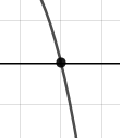
\includegraphics[width=0.3\textwidth]{../Figures/polyZeroBehaviorAA.png}
    \end{center}\begin{enumerate}[label=\Alph*.]
\begin{multicols}{2}
\item 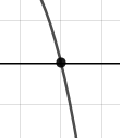
\includegraphics[width = 0.3\textwidth]{../Figures/polyZeroBehaviorAA.png}
\item 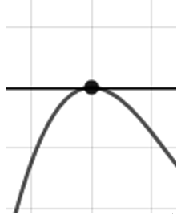
\includegraphics[width = 0.3\textwidth]{../Figures/polyZeroBehaviorBA.png}
\item 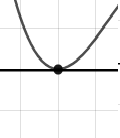
\includegraphics[width = 0.3\textwidth]{../Figures/polyZeroBehaviorCA.png}
\item 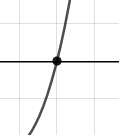
\includegraphics[width = 0.3\textwidth]{../Figures/polyZeroBehaviorDA.png}
\end{multicols}\item None of the above.\end{enumerate}
\textbf{General Comment:} You will need to sketch the entire graph, then zoom in on the zero the question asks about.
}
\litem{
Construct the lowest-degree polynomial given the zeros below. Then, choose the intervals that contain the coefficients of the polynomial in the form $x^3+bx^2+cx+d$.
\[ -2 - 3 i \text{ and } 2 \]The solution is \( x^{3} +2 x^{2} +5 x -26 \), which is option B.\begin{enumerate}[label=\Alph*.]
\item \( b \in [-2.71, -1.5], c \in [3.3, 9.2], \text{ and } d \in [22.8, 26.7] \)

$x^{3} -2 x^{2} +5 x + 26$, which corresponds to multiplying out $(x-(-2 - 3 i))(x-(-2 + 3 i))(x + 2)$.
\item \( b \in [1.42, 2.12], c \in [3.3, 9.2], \text{ and } d \in [-26.6, -24.8] \)

* $x^{3} +2 x^{2} +5 x -26$, which is the correct option.
\item \( b \in [0.14, 1.15], c \in [0.2, 1.1], \text{ and } d \in [-7.3, -4.4] \)

$x^{3} + x^{2} +x -6$, which corresponds to multiplying out $(x + 3)(x -2)$.
\item \( b \in [0.14, 1.15], c \in [-3.6, 0.6], \text{ and } d \in [-4.4, -1.3] \)

$x^{3} + x^{2} -4$, which corresponds to multiplying out $(x + 2)(x -2)$.
\item \( \text{None of the above.} \)

This corresponds to making an unanticipated error or not understanding how to use nonreal complex numbers to create the lowest-degree polynomial. If you chose this and are not sure what you did wrong, please contact the coordinator for help.
\end{enumerate}

\textbf{General Comment:} Remember that the conjugate of $a+bi$ is $a-bi$. Since these zeros always come in pairs, we need to multiply out $(x-(-2 - 3 i))(x-(-2 + 3 i))(x-(2))$.
}
\litem{
Construct the lowest-degree polynomial given the zeros below. Then, choose the intervals that contain the coefficients of the polynomial in the form $ax^3+bx^2+cx+d$.
\[ \frac{-1}{4}, 7, \text{ and } \frac{7}{5} \]The solution is \( 20x^{3} -163 x^{2} +154 x + 49 \), which is option A.\begin{enumerate}[label=\Alph*.]
\item \( a \in [18, 22], b \in [-170, -159], c \in [152, 163], \text{ and } d \in [42, 51] \)

* $20x^{3} -163 x^{2} +154 x + 49$, which is the correct option.
\item \( a \in [18, 22], b \in [106, 113], c \in [-227, -221], \text{ and } d \in [42, 51] \)

$20x^{3} +107 x^{2} -224 x + 49$, which corresponds to multiplying out $(4x -1)(x + 7)(5x -7)$.
\item \( a \in [18, 22], b \in [-178, -171], c \in [231, 239], \text{ and } d \in [-53, -47] \)

$20x^{3} -173 x^{2} +238 x -49$, which corresponds to multiplying out $(4x -1)(x -7)(5x -7)$.
\item \( a \in [18, 22], b \in [159, 164], c \in [152, 163], \text{ and } d \in [-53, -47] \)

$20x^{3} +163 x^{2} +154 x -49$, which corresponds to multiplying out $(4x -1)(x + 7)(5x + 7)$.
\item \( a \in [18, 22], b \in [-170, -159], c \in [152, 163], \text{ and } d \in [-53, -47] \)

$20x^{3} -163 x^{2} +154 x -49$, which corresponds to multiplying everything correctly except the constant term.
\end{enumerate}

\textbf{General Comment:} To construct the lowest-degree polynomial, you want to multiply out $(4x + 1)(x -7)(5x -7)$
}
\litem{
Which of the following equations \textit{could} be of the graph presented below?

\begin{center}
    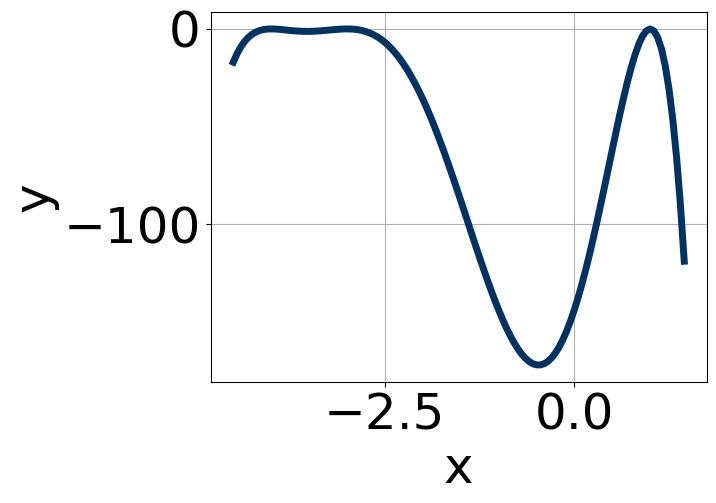
\includegraphics[width=0.5\textwidth]{../Figures/polyGraphToFunctionA.png}
\end{center}


The solution is \( -3(x + 4)^{6} (x + 3)^{6} (x - 1)^{8} \), which is option D.\begin{enumerate}[label=\Alph*.]
\item \( -20(x + 4)^{10} (x + 3)^{5} (x - 1)^{7} \)

The factors $(x + 3)$ and $(x - 1)$ should both have even powers.
\item \( 9(x + 4)^{8} (x + 3)^{8} (x - 1)^{9} \)

The factor $(x - 1)$ should have an even power and the leading coefficient should be the opposite sign.
\item \( 10(x + 4)^{4} (x + 3)^{10} (x - 1)^{6} \)

This corresponds to the leading coefficient being the opposite value than it should be.
\item \( -3(x + 4)^{6} (x + 3)^{6} (x - 1)^{8} \)

* This is the correct option.
\item \( -16(x + 4)^{6} (x + 3)^{4} (x - 1)^{5} \)

The factor $(x - 1)$ should have an even power.
\end{enumerate}

\textbf{General Comment:} General Comments: Draw the x-axis to determine which zeros are touching (and so have even multiplicity) or cross (and have odd multiplicity).
}
\litem{
Describe the zero behavior of the zero $x = 7$ of the polynomial below.
\[ f(x) = -7(x + 7)^{5}(x - 7)^{10}(x - 4)^{4}(x + 4)^{7} \]The solution is the graph below, which is option B.
    \begin{center}
        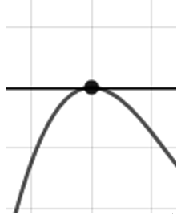
\includegraphics[width=0.3\textwidth]{../Figures/polyZeroBehaviorCopyBA.png}
    \end{center}\begin{enumerate}[label=\Alph*.]
\begin{multicols}{2}
\item 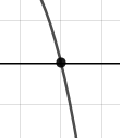
\includegraphics[width = 0.3\textwidth]{../Figures/polyZeroBehaviorCopyAA.png}
\item 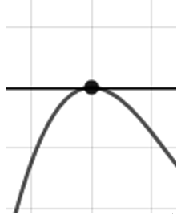
\includegraphics[width = 0.3\textwidth]{../Figures/polyZeroBehaviorCopyBA.png}
\item 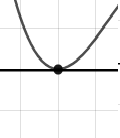
\includegraphics[width = 0.3\textwidth]{../Figures/polyZeroBehaviorCopyCA.png}
\item 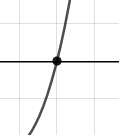
\includegraphics[width = 0.3\textwidth]{../Figures/polyZeroBehaviorCopyDA.png}
\end{multicols}\item None of the above.\end{enumerate}
\textbf{General Comment:} You will need to sketch the entire graph, then zoom in on the zero the question asks about.
}
\end{enumerate}

\end{document}